\chapter{Implementation}
% Implementation-introtekst
This chapter gives an overview of the developed musical multi-robot system. The main goal of the implemented system is to allow for a multi-robot (musical) collective to interact with each other in order to achieve emergent and co-ordinating/co-operative behaviour—synchronization specifically in our case—with varying degrees of difficulty and certainty in the environment and communication. More specifically, the goal with the design is to enable the robot collective to achieve so-called \textit{harmonic synchronization} \inkl{within a relatively short time, much depending on the design parameters and environment conditions}. What is meant by \textit{harmonic synchronization} will be expounded in Subsection \ref{subsec:harmonic_synchrony}. These goals firstly require of the agents/nodes the modelling of oscillators with their properties, like phase and frequency, as explained further in Subsection \ref{subsec:node}. To allow for interaction and communication between the agents, mechanisms so that the agents can transmit "fire"-signals, as well as listen for other agents's "fire"-signals, is necessary as well, and is presented in Subsection \ref{subsec:fire_signal}.






% Fake seksjon med alle relevante concerns (FJERN HVIS DU SKAL FÅ FEEDBACK FRA KYRRE)
\tcol[gray]{\section{(Fake seksjon) Betraktninger:}}
\besk{"Det man har utviklet" — Kyrre}
\besk{"Det er her man henter fisken tilbake på land (blant andre steder — som f.eks. der man dokumenterer eksperimentene sine godt)."ish — Jim}

\gjor{Skriv opp Worklog-materiale (under ``muy bien so far''-bokmerket) dandert i henhold til gode master-theses}

\gjor{
	\textbf{Svar på disse spørsmålene (kompilert fra Tønnes sin masteroppgave):}
	What does the chapter do? What's the main goal of the design/implementation/developed system? What do these goals require? Why did you make the design-choices you made? What advantages do these choices ensure/enable? Give a short chapter-outline (perhaps first about the design, my additional Self-Awareness component, manual choice of initial parameters, and then the benchmark or målestokk or performance measure I use to evaluate with).
}

\gjor{Se på Tønnes sin Masteroppgave og 'Archive History'-kommentarene nederst i .tex-fila for inspirasjon}







% Seksjon om baselinen (hva jeg baserer min implementasjon på, forskjellig fra mitt eget bidrag)
\section{The baseline: Achieving Decentralized Harmonic Synchronization in (Oscillators $\vee$ Musical Robot Collectives)}
	\label{sec:baseline}
	\besk{Nymoens ideer og algoritmer implementert i mitt system i Unity}

	Envision that we have a multi-agent collective scenario consisting of musical robots modelled as oscillators, solely communicating through brief ``fire''-like audio-signals|greatly inspired by K. Nymoen et al.'s approach for achieving \textit{decentralized harmonic synchronization in mobile music systems} \cite{nymoen_synch}. These agents are initially not synchronized in their firing of audio-signals, but as time goes, they are entraining to synchronize to each other by adjusting their phases and frequencies when or after hearing each other's audio-signals. An illustration of this is given in Figure \ref{fig:initial}.

	% First Intro-illustration figure to easily get a quick idea of what the system/design does/consists of:
	\begin{figure}[h]
		\centering
			\begin{subfigure}[t]{.5\textwidth}
				\centering\captionsetup{width=.9\linewidth}%
				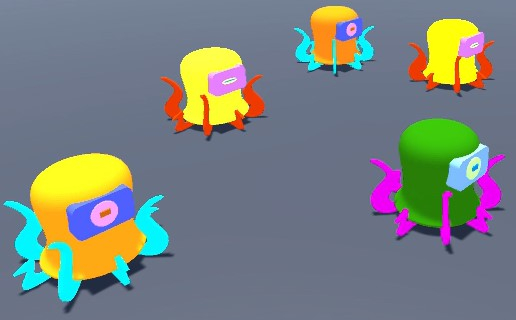
\includegraphics[width=0.9\linewidth]{Assets/Figures/IntroUnsynch.jpg}
				\caption{The agents firing asynchronously at first. Here, only the two Dr. Squiggles with red tentacles are firing simultaneously, but the rest are not.}
				\label{fig:initial:unsynch}
			\end{subfigure}%
			\begin{subfigure}[t]{.5\textwidth}
				\centering\captionsetup{width=.9\linewidth}%
				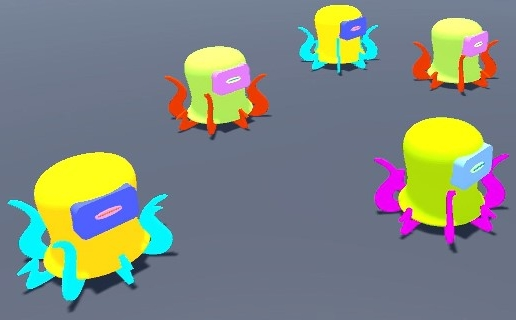
\includegraphics[width=0.9\linewidth]{Assets/Figures/IntroSynch.jpg}
				\caption{Seconds later, after having listened to each other's fire-event signals and adapted themselves accordingly, the agents are here firing synchronously.}
				\label{fig:initial:synch}
			\end{subfigure}
		\caption{Decentralized Synchronization of phases achieved in a musical robot collective, consisting of M. J. Krzyzaniak and RITMO's Dr. Squiggles. \tcol{(NB! Dette skaper kanskje en misoppfatning om at alle noder må fyre samtidig for å være synkroniserte.. Husk at dette ikke er tilfellet med \textit{harmonisk synkronisering}. \inkl{denne figuren} Husk også tvetydigheten med den orange Dr. Squiggle'n og den gule ``fire''-color'en, og at du nå bruker .JPG (æsj))}}	% Gammel caption: "The musical agents, also known as M. J. Krzyzaniak's Dr. Squiggles, are actively listening for signals from each other's fire-events, entraining to synchronize to each other accordingly." Cite Pierre her? Nevne Phase-adjustments også her?
		\label{fig:initial}
	\end{figure}

	These aforementioned audio-signals to be expounded further in Subsection \ref{subsec:fire_signal}, also referred to as ``fire''-signals, are transmitted whenever an agent's oscillator \textit{peaks} (i.e. after its cycle or period is finished, having phase $\phi(t)=1$)|or actually every second \textit{peak}, due to the target system goal of \textit{harmonic synchrony}. All agents have the ability to listen for such transmitted ``fire''-signals from their neighbours, which they then will use as a trigger to adjust themselves according to some well-designed update-functions to be elaborated in Subsection \ref{subsec:update_functions}.

	\gjor{Insert a phase-/time-plot Figure with two Subplots. Subplot 1: phase-/time-plot when oscillators are unsynchronized. Subplot 2: phase-/time-plot when oscillators are synchronized}
	\gjor{Insert a frequency-/time-plot Figure with two Subplots. Subplot 1: frequency-/time-plot when oscillators are unsynchronized. Subplot 2: frequency-/time-plot when oscillators are synchronized}


	% SUBSEKSJONER TIL BASELINE-SEKSJONEN:

	% Subseksjon om den enkelte noden/agenten med alle egenskaper den har osv.
	\subsection{The node: the musical robot individual}
	\label{subsec:node}
	\besk{Subseksjon om den enkelte noden/agenten med alle egenskaper den har osv. (som f.eks. en oscillator-komponent (jf. Nymoens Implementation-seksjon))}

	% Subseksjon om kommunikasjonsmetoden til agentene: audio-/``fire''-signalet
	\subsection{Robot communication: the ``fire''-signal}
	\label{subsec:fire_signal}
	\besk{Subseksjon om kommunikasjonsmetoden til agentene: audio-/``fire''-signalet}

	% Subseksjon om target-staten til systemet: harmonisk synkroni
	\subsection{System target state: Harmonic Synchrony}
	\label{subsec:harmonic_synchrony}
	\besk{Subseksjon om target-staten til systemet: harmonisk synkroni}
	The goal and target state of the system is \textit{harmonic synchrony}, as K. Nymoen et al. \cite{nymoen_synch} coined it when ...
	
	% Subseksjon om update-functions for frekvens- og fase-oppdateringene
	\subsection{Update functions: Phase- \& Frequency-Adjustment}
	\label{subsec:update_functions}
		\subsubsection{Phase Adjustment}
		If we assume constant and equal oscillator frequencies in our agents, we can first take a look at how the agents adjust their phase in order to synchronize to each other.
		
		\gjor{1) Insert det om ``standard'' phase-adjustment, sånn som Mirollo \& Strogatz gjorde det \cite{}, med passende figurer og illustrasjoner}
		
		\gjor{2) Insert det om ``bi-directional'' phase-adjustment, sånn som K. Nymoen et al. gjorde det \cite{nymoen_synch}, med passende figurer og illustrasjoner}
		
		
		
		\subsubsection{Frequency Adjustment}
		\gjor{Presenter hva Frequency-adjustment er (hvis det ikke ble tydelig nok i slutten av Seksjon-\ref{sec:baseline}), bygg opp fremgangsmåten på hvordan man oppnår Frequency-adjustment (som i reMarkable-notatet 'Logs' $\rightarrow$ 'Simulations' $\rightarrow$ 'Frequency adjustment', og Worklog'en) | med passende figurer og illustrasjoner}









% Seksjon om mitt bidrag (skill tydelig på mine bidrag og det jeg ikke har gjort noe med)
\section{The new proposed algorithm: an additional Self-Awareness component}









% Archive History:

	% \section{Benchmark}
		% \besk{Her jeg beskriver Nymoens algoritmer og formler (originalt), men \opphoy{sånn jeg har implementert det i Unity}}
	
		% \gjor{Vurder om 'Benchmark' bør deles opp i sin egen sub-seksjon i det hele tatt — eller f.eks. slås sammen med 'Proposed Algorithm'}
	
		% \besk{(Hentet fra Samuelsens master?) Presentering av metoden brukt til å evaluere ytelsen av den foreslåtte/proposed'e algoritmen. Først er kanskje en referanse-algoritme brukt for sammenlikning beskrevet. Deretter er (f.eks. objektiv-) funksjoner brukt i testene forklart. Endelig (til slutt) er kanskje miljøene/environments'a og parameterne brukt presentert}
		
		
	% \section{Proposed Algorithm}
		% \besk{Evt. her jeg skriver om Self-Awareness-komponenten(e) jeg legger til ang. Belief-awareness og/eller Expectation-awareness (jf. det jeg og Kyrre snakka om Mid-November på 'reMarkable -> Møter -> ROBIN -> Kyrre')}
	
		% \gjor{Vurder om 'Proposed Algorithm' bør deles opp i sin egen sub-seksjon i det hele tatt — eller f.eks. slås sammen med 'Benchmark'}
	